\documentclass{article}
\usepackage[a4paper,margin=1in]{geometry}
\usepackage{amsmath}
\usepackage{graphicx}
\usepackage[colorlinks=true, allcolors=blue]{hyperref}
\usepackage{tikz}
\usepackage{gensymb}
\usepackage{float}


\pagenumbering{arabic}
\title{IB2\\Verslag 1}
\date{11/10/2023}
\author{Tom Thys, Daan Vercammen, Sander Haustraete}

\begin{document}
\maketitle

\begin{minipage}{\textwidth}
    \centering
    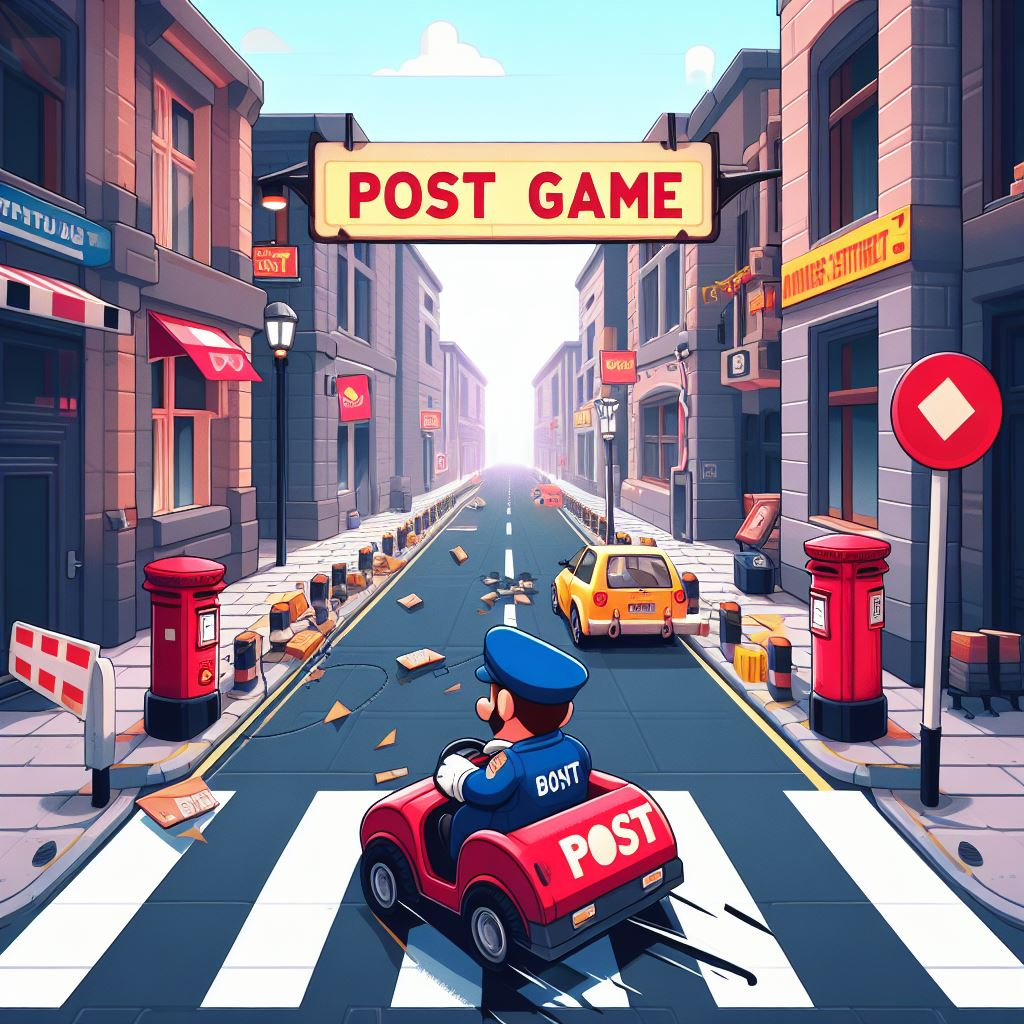
\includegraphics[width=0.7\textwidth]{fotos/_a1a1db80-3fb5-41c9-9da6-cb8f494513cb.jpg}
\end{minipage}

\vspace{50pt}

\begin{minipage}{\textwidth}
    \centering
    
\includegraphics[width=0.5\textwidth]{fotos/Logo.png}

\end{minipage}

\newpage


\section{Doel en doelgroep}
\subsection{Doel}
Het doel van het spel is vrij simpel, breng als postbode in 1 minuut zoveel mogelijk pakjes naar de juiste plaats. Dit doe je 
door rond te rijden in een lange straat. Op je scherm zie je een gps die je de juiste richting aangeeft. Wanneer je op het juiste adres
bent, brengt de gps je naar je nieuwe locatie. Maar het is natuurlijk niet gewoon van punt a naar punt b rijden. De straat staat namelijk
vol met obstakels zoals bomen en vuilnisbakken. En er rijden natuurlijk ook andere auto's rond in de straat. Wanneer je tegen een van 
die obstakels of andere auto's botst is het game over. Je moet dus zonder te botsen zo rap mogelijk en zo veel mogelijk pakjes 
bezorgen. Zou jij de highscore kunnen halen? 
\subsection{Doelgroep}
Door het simpel en duidelijk concept is het spel geschikt voor een zeer breed publiek. We vermoeden toch dat het vooral zou aanslaan 
bij kinderen. Maar toch is het ook een spel dat we zelf zouden kunnen spelen als we wat afleiding nodig hebben zonder veel te moeten 
nadenken.
\section{Overview and features}
\subsection{Uitdagingen}

\subsubsection{GPS}
Het toevoegen van een gps leek ons een leuke uitdaging. Via de gps zou je altijd in staat moeten zijn om te zien waar je naartoe moet.
\subsubsection{Oneindig}
Het leek ons ook een leuk idee om de wereld oneindig te maken. Dit zorgt natuurlijk voor extra uitdagingen op het vlak van navigatie en 
de snelheid van de game.
\subsubsection{Collision detection objecten}
Wanneer de auto botst tegen 1 van de obstakels moet het spel worden afgesloten.
\subsubsection{Advanced texture}
Het is de bedoeling dat de texture bestaat uit verschillende soorten huizen, waardoor de game iets realistischer wordt.


\subsection{Extra's}
Wanneer we tijd over hebben kunnen we natuurlijk altijd nadenken over extra's om de game nog beter te maken. Zo zou je bijvoorbeeld 
achtervolgd kunnen worden door een politiewagen wanneer je tegen iets botst. In dat geval zou het dus niet meteen game over zijn, 
maar kun je nog proberen vluchten. Het zou ook mogelijk zijn meer variatie in de map te steken in plaats van enkel 1 lange straat. 
Wat ook zou kunnen is dat we het mogelijk maken andere objecten te vernietigen voor extra punten. We hebben dus nog een aantal opties 
om de game te avenceren indien nodig.


\end{document}